%%
%% Qbe SAS SystemDocumentation
%% (C) Copyright 2001-2004 Christian Hofstaedtler
%%
%% $Id: part-last.tex 20 2004-05-03 15:41:20Z ch $
%%

\cChapter{Netzwerk�bersicht HTL}
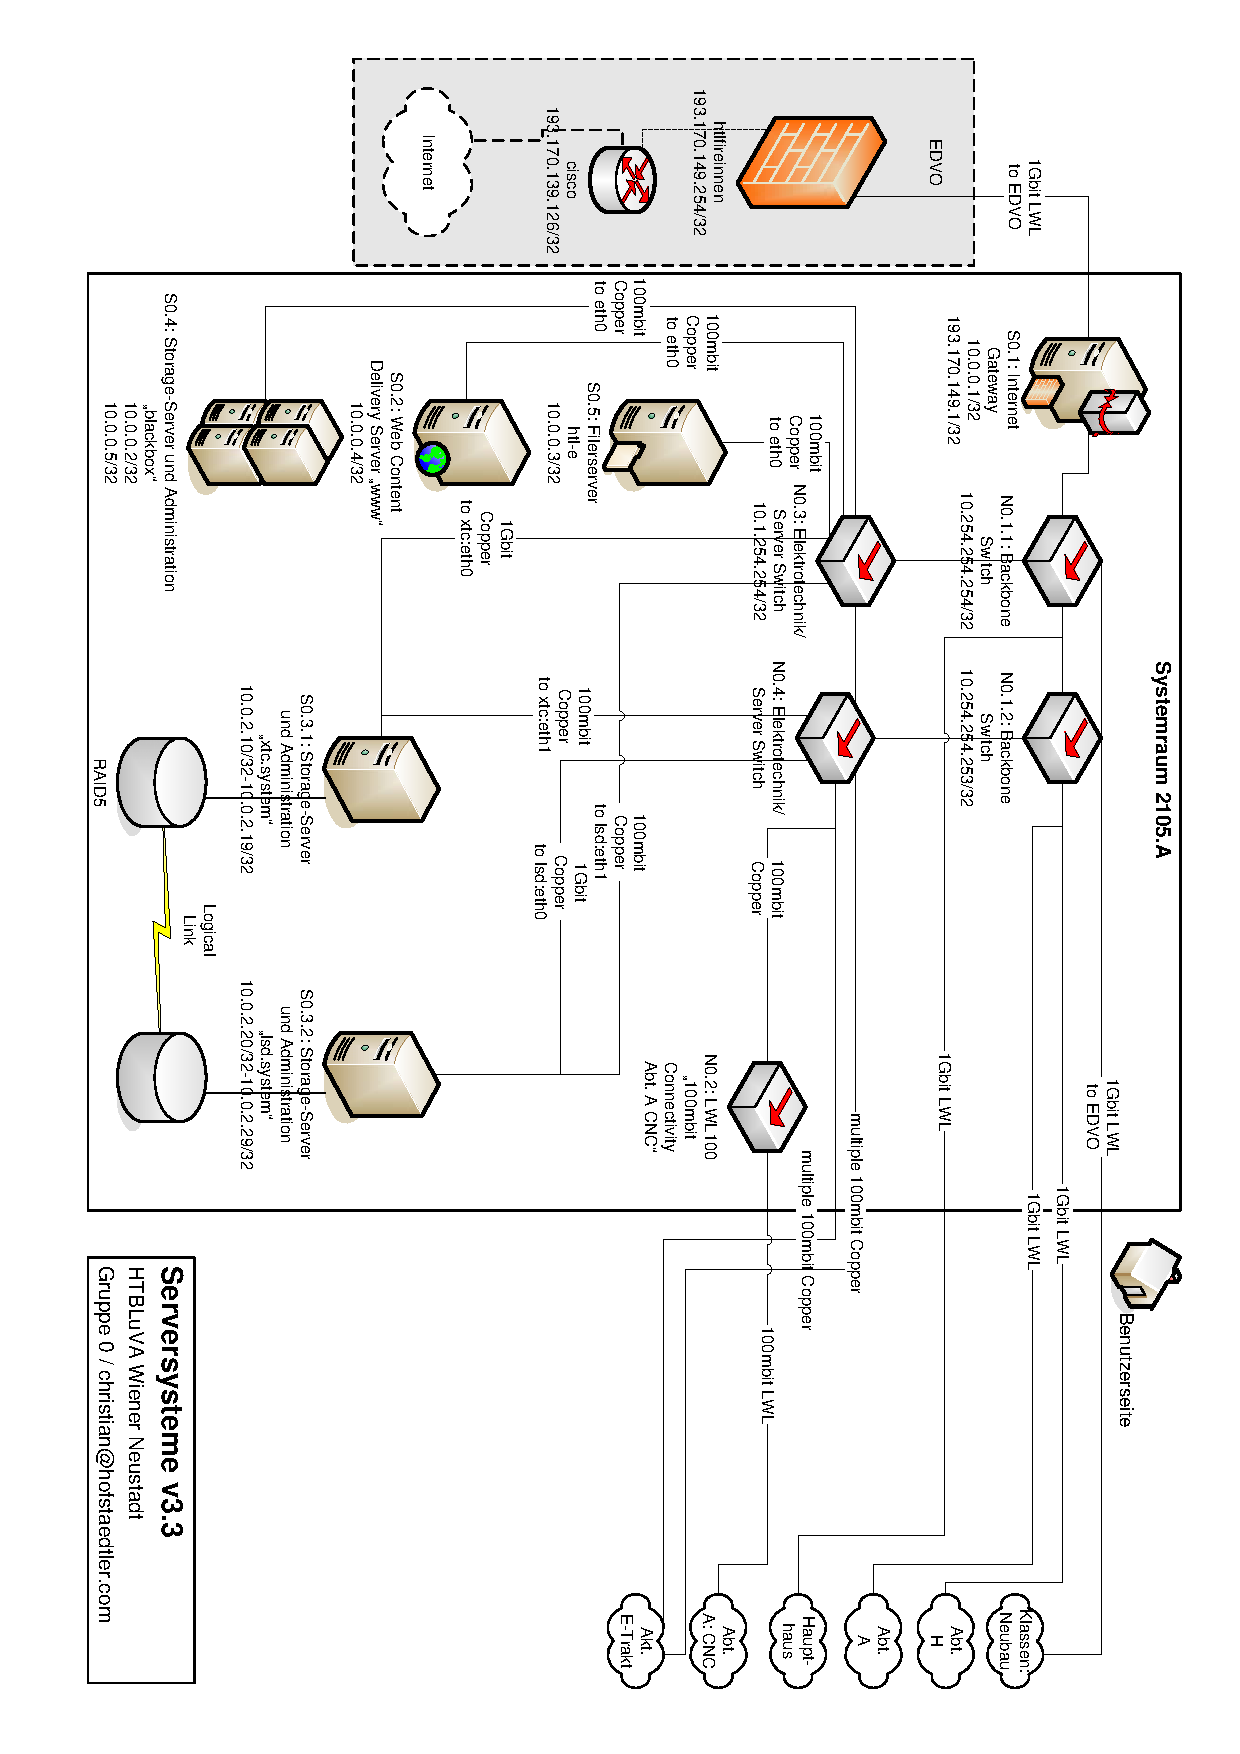
\includepdf[pages={1}]{files/htl-net-struct.pdf}
%\{htl-net-struct.pdf}{HTL Netzwerkstruktur}

\cChapter{HTL eDirectory Struktur}
\begin{landscape}
Im folgenden findet sich eine �bersicht des eDirectory Verzeichnisses. Hier mit Treename "HTL" und Basiskontext "o=htlwrn,c=at".

Der Kontext "o=System" ist nicht via LDAP sichtbar, kann daher auch nicht einfach von Applikationen ver�ndert/besch�digt werden.

\placefig{htl-nds-struct}{HTL eDirectory Struktur}

FIXME: Administration Container zeichnen.

\par

\section{Neue eDirectory Attribute}

inetStatus, loggedonHost, loggedonMac, traffic und lastActivity werden in den Benutzer-, Gruppen-, Klassen-, und Computer-Objekten verwendet. Die qbePolicy*-Attribute werden nur f�r die Computer-Policy-Objekte (qbeHostPolicy) verwendet.

\begin{lstlisting}
attributeTypes: ( 1.2.826.0.1.16224.0.0.0.10 NAME 'inetStatus' SYNTAX 1.3.6.1.4.1.1466.115.121.1.27 SINGLE-VALUE )
attributeTypes: ( 1.2.826.0.1.16224.0.0.0.11 NAME 'loggedonHost' SYNTAX 1.3.6.1.4.1.1466.115.121.1.15{64512} SINGLE-VALUE )
attributeTypes: ( 1.2.826.0.1.16224.0.0.0.12 NAME 'loggedonMac' SYNTAX 1.3.6.1.4.1.1466.115.121.1.15{128} SINGLE-VALUE )
attributeTypes: ( 1.2.826.0.1.16224.0.0.0.13 NAME 'traffic' SYNTAX 1.3.6.1.4.1.1466.115.121.1.36{64512} SINGLE-VALUE )
attributeTypes: ( 1.2.826.0.1.16224.0.0.0.14 NAME 'lastActivity' SYNTAX 1.3.6.1.4.1.1466.115.121.1.27 SINGLE-VALUE )
attributeTypes: ( 1.2.826.0.1.16224.0.0.0.15 NAME 'qbePolicyDynamicUserGroup' SYNTAX 1.3.6.1.4.1.1466.115.121.1.15{64512} )
attributeTypes: ( 1.2.826.0.1.16224.0.0.0.16 NAME 'qbePolicyDynamicUserEnabled' SYNTAX 1.3.6.1.4.1.1466.115.121.1.27 SINGLE-VALUE )
attributeTypes: ( 1.2.826.0.1.16224.0.0.0.17 NAME 'qbePolicyName' SYNTAX 1.3.6.1.4.1.1466.115.121.1.12 )
attributeTypes: ( 1.2.826.0.1.16224.0.0.0.18 NAME 'qbePolicyLoginScript' SYNTAX 1.3.6.1.4.1.1466.115.121.1.15{64512} SINGLE-VALUE )
attributeTypes: ( 1.2.826.0.1.16224.0.0.0.19 NAME 'qbePolicyHomeDrive' SYNTAX1.3.6.1.4.1.1466.115.121.1.15{64512} SINGLE-VALUE )
attributeTypes: ( 1.2.826.0.1.16224.0.0.0.20 NAME 'qbePolicyHomeDriveDir' SYNTAX 1.3.6.1.4.1.1466.115.121.1.15{64512} SINGLE-VALUE )
\end{lstlisting}

Bei einer Neuinstallation sollten die Attribute inetStatus, loggedonHost, loggedonMac, traffic und lastActivity auf qbe* umbenannt werden. Dies w�rde die Schemaverwaltung vereinfachen, zieht jedoch auch �nderungen in den PHP Skripten nach sich.


\section{Neue eDirectory Objekte}

qbeOrganizationalUnit und qbeGroup werden f�r die Klassen-/Gruppen-Verwaltung verwendet. qbeIpDevice, qbeOwnedObject und qbeHostPolicy f�r die ComputerVerwaltung.

\begin{lstlisting}
objectClasses: ( 1.2.826.0.1.16224.0.0.0.1 NAME 'qbeOrganizationalUnit' SUP organizationalUnit AUXILIARY MAY ( cn $ inetStatus ) X-NDS_NOT_CONTAINER '1' )
objectClasses: ( 1.2.826.0.1.16224.0.0.0.2 NAME 'qbeGroup' SUP groupOfNames AUXILIARY MAY inetStatus X-NDS_NOT_CONTAINER '1' )

objectClasses: ( 1.2.826.0.1.16224.0.0.0.3 NAME 'qbeIpDevice' AUXILIARY MAY ( macAddress $ ipHostNumber $ qbePolicyName ) X-NDS_NOT_CONTAINER '1' )
objectClasses: ( 1.2.826.0.1.16224.0.0.0.4 NAME 'qbeOwnedObject' AUXILIARY MAY owner X-NDS_NOT_CONTAINER '1' )
objectClasses: ( 1.2.826.0.1.16224.0.0.0.5 NAME 'qbeHostPolicy' AUXILIARY MUST qbePolicyDynamicUserEnabled MAY ( qbePolicyDynamicUserGroup $ qbePolicyHomeDrive $ qbePolicyHomeDriveDir $ qbePolicyLoginScript ) X-NDS_NOT_CONTAINER '1' )
\end{lstlisting}

\end{landscape}


\cChapter{Cluster-Installation HTL}

Der HTL-Cluster f�r den Authentication Server besteht aus zwei identischen Intel-Servern. Der Cluster-Name lautet auf qbe-auth.htlwrn.ac.at. Die Intel-Server wurden xtc.system.htlwrn.ac.at (Prim�rer Server) und lsd.system.htlwrn.ac.at (Sekund�rer Server) getauft.

Als Cluster Monitor-Software wird heartbeat eingesetzt. Die Intel-Server sind vom Modell SR2300 und mit dem Intel SE7501WV2 sowie dem Intel Raid-Controller SRCZCR ausgestattet.

Novell eDirectory wird nicht vom heartbeat verwaltet, es l�uft immer auf beiden Cluster Nodes. Alle anderen Dienste werden vom heartbeat gestartet/gestoppt.

Die Cluster-Applikationen und IP-Adressen:
\begin{description}
\item[Filesystem::/dev/nb0::/raid::ext3::noatime,usrquota,grpquota]{Das /raid (Daten-)Dateisystem}
\item[qbe-sas-daemon]{Hintergrunddienste vom Application Server}
\item[10.0.2.100]{Application Server IP}
\item[172.16.0.1/16]{Application Server IP f�r unbekannte Clients}
\item[apache::/etc/apache/httpd.conf]{Application Server Webserver}
\item[samba]{CIFS Server}
\item[mysql]{SQL Server}
\item[vsftpd]{FTP Server}
\item[nfs-kernel-server]{Network File System (NFS) Server f�r die www}
\item[dhcp3-server]{DHCP Server}
\item[10.0.2.104]{SubVersion IP}
\item[apache2]{SubVersion Server}
\end{description}


%% *eof*
